\documentclass[12pt]{article}
\usepackage[brazil]{babel}
\usepackage[a4paper, total={6.5in, 9.5in}]{geometry}
\usepackage[utf8]{inputenc}

\usepackage{authblk}
\usepackage{lipsum}
\usepackage{xcolor}
\usepackage{listings}
\usepackage[normalem]{ulem}
\usepackage{amssymb}
\usepackage{float}
\usepackage{graphicx}
\usepackage{amsmath}
\usepackage{amsthm}
\usepackage{amssymb}
\usepackage{verbatimbox}
\newtheorem{theorem}{Theorem}[section]
\newtheorem{lemma}[theorem]{Lemma}

\definecolor{codegreen}{rgb}{0,0.6,0}
\definecolor{codegray}{rgb}{0.5,0.5,0.5}
\definecolor{codered}{rgb}{0.8,0,0}
\definecolor{backcolour}{rgb}{0.95,0.95,0.92}

\usepackage{inconsolata}
\lstset{
    language=python,
    backgroundcolor=\color{backcolour},   
    commentstyle=\color{codegreen},
    keywordstyle=\color{blue},
    numberstyle=\tiny\color{codegray},
    stringstyle=\color{codered},
    basicstyle=\ttfamily\small,
    numberstyle=\footnotesize,
    numbers=left,
    backgroundcolor=\color{white},
    frame=single,
    tabsize=2,
    rulecolor=\color{white},
    title=\lstname,
    escapeinside={\%*}{*)},
    breaklines=true,
    breakatwhitespace=true,
    framextopmargin=2pt,
    framexbottommargin=2pt,
    inputencoding=utf8,
    extendedchars=true,
    showstringspaces=false,
    literate={á}{{\'a}}1 {ã}{{\~a}}1 {é}{{\'e}}1 {Ó}{{\'O}}1 {Ã}{{\~A}}1 {í}{{\'i}}1 {ó}{{\'o}}1 {ç}{{\.c}}1 {ê}{{\^e}}1 {ú}{{\'u}}1,
}

% \pagecolor[rgb]{0.1,0.1,0.1} %black
% \color[rgb]{0.75,0.75,0.75} %grey

\title{\textbf{Segurança Computacional\\ \Large{Geração e Verificação de Assinatura Digital}}}
\author{Pedro Henrique de Brito Agnes, 18/0026305
\\ Pedro Pessoa Ramos, 18/0026488
}
\affil{Dep. Ciência da Computação - Universidade de Brasília (UnB) \vspace{-2ex}}
\date{}

\begin{document}
\maketitle

\section{Implementação}

Foi desenvolvido um algoritmo em python na versão 3.8 ou acima que recebe um arquivo e gera a assinatura digital para ele ou verifica a assinatura. Para executar passando o documento \texttt{msg.txt} e produzindo o resultado em \texttt{sample/cifra.txt}, pode-se usar o comando abaixo:

\begin{lstlisting}
python src/signature.py sample/msg.txt -o sample/cifra.txt
\end{lstlisting}

Vão ser geradas as chaves pública e privada do RSA que foram usadas para a cifração do hash (assinatura) e da chave de sessão (AES), que será gerada também, contendo a original em um arquivo e a sua cifra em outro. O programa vai avisar o local e nome de cada uma das chaves geradas. Pode ser passado o argumento \texttt{-h} para o programa para a listagem de opções disponíveis conforme mostrado abaixo:

\begin{itemize}
    \item \textbf{-o} - Onde será feito o output. Obrigatório
    \item \textbf{-k} - Arquivo com a chave pública ou privada, a depender da operação. Obrigatório na decifração.
    \item \textbf{-s} - Arquivo com a chave de sessão ou o criptograma da chave de sessão. Obrigatório na decifração.
    \item \textbf{-d} - Argumento que indica que o programa vai descriptografar. Deve ser passado no final do comando sem parâmetros adicionais.
\end{itemize}

Por exemplo, para cifrar o arquivo \texttt{sample/msg.txt} com a chave de sessão encontrada no arquivo \texttt{keys/session\_sample} gerar a sua assinatura digital com a chave privada localizada em \texttt{keys/key\_sample} e armazenar o criptograma da mensagem no arquivo \texttt{sample/cifra.txt}, pode ser usado o comando abaixo:

\begin{lstlisting}
python src/signature.py sample/msg.txt -s keys/session_sample -k keys/key_sample -o sample/cifra.txt
\end{lstlisting}

Além do argumento passado para o \texttt{-o}, será gerado um outro arquivo de mesmo nome concatenado com \texttt{\_sign} que representa a assinatura. Este arquivo não precisará ser passado ao programa, ele será encontrado automaticamente ao passar o \texttt{-o} ao usar a opção de decifrar.

Da mesma forma, para decifrar o criptograma gerado com a chave de sessão cifrada \texttt{keys/session\_sample.pub} e armazenar o resultado em um arquivo \texttt{sample/out.txt}, pode-se usar o comando abaixo que utiliza a chave privada:

\begin{lstlisting}
python src/signature.py sample/cifra.txt -s keys/session_sample.pub -k keys/key_sample.pub -o sample/out.txt -d
\end{lstlisting}

Após a finalização da execução, o programa vai informar se o hash gerado após as operações é igual ao hash obtido anteriormente, ou seja, vai verificar se a assinatura é válida.

\section{RSA}
\subsection{Geração de Chaves}

Inicialmente são gerados 2 números primos aleatórios \texttt{p} e \texttt{q} de 1024 bits cada. Para obter estes números, foi inicialmente gerado um número qualquer do tamanho especificado, em seguida, sua primalidade foi testada para cada um dos primos até 1000, que foram dispostos em um array após serem computados uma única vez pelo crivo de Erastótenes. Em seguida, é realizado o teste de primalidade probabilístico de Miller Rabin, executado 20 vezes. Se ambos os testes passarem, o número é considerado primo e selecionado. Caso contrário, um novo número aleatório é gerado para realizar o teste novamente. Os códigos relacionados à geração e verificação dos primos estão localizados na pasta \texttt{src/util/primes.py}, incluindo a implementação do algoritmo de Miller Rabin.

Com \texttt{p} e \texttt{q} definidos, a chave pública é obtida usando 2 valores, o \texttt{n} e o \texttt{e}. O número \texttt{n} é o resultado da multiplicação de \texttt{p} e \texttt{q}, logo sendo de 2048 bits e já o \texttt{e} será um primo bem menor que \texttt{p} e \texttt{q}. Já a chave privada é obtida pela função totiente de Euler em \texttt{n}, onde temos a multiplicação de 2 números primos, logo, podendo ser calculada pela fórmula abaixo:

\[
    \phi(n) = (p-1) \times (q-1)
\]

Com o resultado da função acima, é calculado o seu inverso multiplicativo com \texttt{e} para assim obter o valor de \texttt{d} que é o único valor necessário para a chave privada. Para fins de performance, também são adicionados os valores de \texttt{p} e \texttt{q} na chave privada. Após a geração, as chaves são guardadas na pasta \texttt{keys} com a formatação base64, sendo a pública com a extensão \texttt{.pub}.

\subsection{Cifragem e Decifragem}

Como trata-se da assinatura digital, é usada a chave privada para cifrar e a pública para decifrar, sendo o contrário do RSA "convencional". Para cifrar, é feita simplesmente uma potenciação entre a mensagem (bytes concatenados em um número gigante) e o valor de \texttt{d}, onde é pego o resto da divisão por \texttt{n}. Já para decifrar, é feita a potênciação da mensagem com \texttt{e}, também pegando o resto da divisão por \texttt{n}.

No programa, o que é cifrado pelo RSA é o hash do criptograma da mensagem gerado pelo AES, resultando na assinatura digital e em seguida, a chave de sessão que foi usada no AES. Para a verificação, a assinatura é decifrada para assim obter o hash, e em seguida, esse hash é comparado com o hash gerado pelo criptograma que foi recebido e o programa informa se os hashs são iguais. Também é decifrada a chave de sessão para que a mensagem original seja recuperada. Os arquivos relacionados à implementação RSA podem ser encontrados na pasta \texttt{src/rsa/}.

\section{AES}

O AES foi usado no modo CTR com o nonce fixo no valor 0 para a cifração simétrica da mensagem, que é usada para gerar o hash, sendo usada a chave de sessão para cifrar e decifrar. A implementação da cifra de blocos foi aproveitada do trabalho anterior da disciplina de segurança computacional, podendo ser econtrada na pasta \texttt{src/aes/}.

A geração da chave é feita na pasta \texttt{keys/}, sendo nomeada \texttt{session} e concatenada com um id incremental. Consequentemente, será gerado o arquivo de mesmo nome porém com a extensão \texttt{.pub} que representa a mesma chave porém cifrada pelo RSA e é a usada na verificação da assinatura, porém deve ser decifrada antes de ser utilizada. 

\section{Assinatura}

Para a assinatura, foi criado um hash do criptograma gerado pelo AES usando a função \texttt{sha3\_256} da \texttt{hashlib} diponibilizada pela linguagem python. Para a formatação dos valores ao escrevê-los em arquivos, foi usado o \texttt{base64}, que é disponibilizado pelo python também, dispondo de operações para codificar e decodificar no formato. A assinatura do documento é gerada em um arquivo separado que tem o mesmo nome do output (criptograma da mensagem) concatenado com um \texttt{\_sign}. A implementação completa pode ser resumida às imagens abaixo:

\begin{figure}[H]
	\centering
    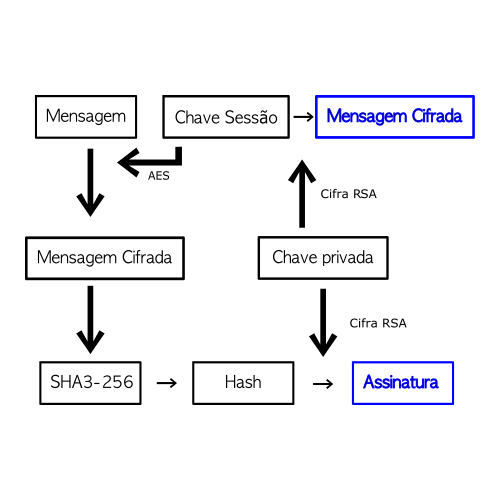
\includegraphics[width=.65\textwidth]{img/assinatura.png}
    \caption{Geração da assinatura}
\end{figure}

\begin{figure}[H]
	\centering
    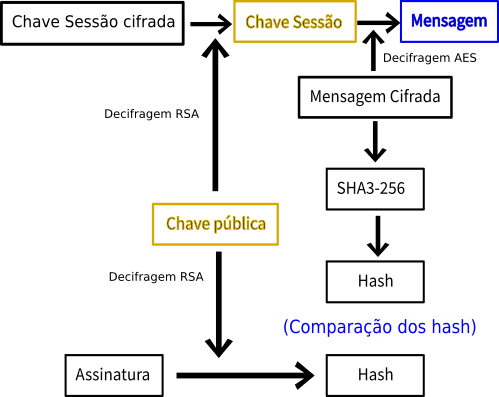
\includegraphics[width=.65\textwidth]{img/verificacao.png}
    \caption{Verificação da assinatura}
\end{figure}

\section{Conclusões}

Com a assinatura do documento, ao cifrá-lo e enviar a outra pessoa com as chaves necessárias, fica mais fácil de se verificar a integridade, pois qualquer mínima alteração no documento gerará um hash diferente que será identificado na verificação. O RSA é um grande nome no ramo das assinaturas digitais, sendo muito usado para a cifração do hash, já que é um algoritmo assimétrico e permite o envio apenas da cahve pública para o recipiente, o que impede de que seja gerada uma assinatura falsa.

\end{document}
